\documentclass[../main.tex]{subfiles}


\begin{document}

\chapter{Protocol design}
\label{chap:design}

This chapter describes and justifies the protocol designed in the context of this thesis.
The main purpose of the protocol is the secure encryption of logs in the toolchain.
In the previous chapter \ref{chap:overview}, possible encryption strategies were introduced and evaluated based on the identified system requirements in chapter \ref{chap:requirements}.
Hybrid encryption was identified as the most promising encryption technique.
The evaluation of the protocol in terms of functionality, security, and performance can be found in chapter~\ref{chap:evaluation}.
A high-level overview of the designed protocol can be found in section~\ref{sec:overview}.
Section~\ref{sec:protocol-considerations} reflects different design considerations for the protocol.
The imposed algorithms to create, encrypt and decrypt logs are explained in the subsequent sections. 

\section{Protocol overview}
\label{sec:overview}

The implemented protocol extends the current toolchain because it supports encrypted logs.
Additionally, access to encrypted logs can be shared and revoked by the data owner of a log.

The protocol relies on a PKI.
Each user requires two key pairs.
One key pair is dedicated to encrypting data.
The second key pair is intended to sign data.
This separation of keys is considered to be the best practice in modern key management.~\todo{quelle}
Each user needs to have exclusive access to its private keys.
The public keys of all users are expected to be publicly available in the system.

The protocol relies on three fundamental operations: 
Creating, encrypting and decrypting logs.
This procedure sketched in the following is visualized in figure~\ref{fig:protocol-overview}.
Whenever a monitor component observes a data access it creates an access log.
The log is not a plain data structure.
Rather, a log must always be signed by the monitor that created it.
Thus, the protocol requires the monitor to perform two tasks.
First, the raw log data needs to be cryptographically signed by the monitor.
Second, the log needs to be encrypted for the data owner (only the data owner is allowed to access the log upon creation).
The encrypted log is finally sent to the Overseer.
This allows the data owner to request and decrypt the log.
The decryption process also involves validity checks of the received data.
The data owner can share or revoke access to the log for users.
This requires the data owner to apply the encryption algorithm and upload the re-encrypted data to the Overseer.
All specified receivers can download and decrypt the log.
Again, validity checks of the received data ensure that the defined security requirements are respected.

\begin{figure}[h!]
    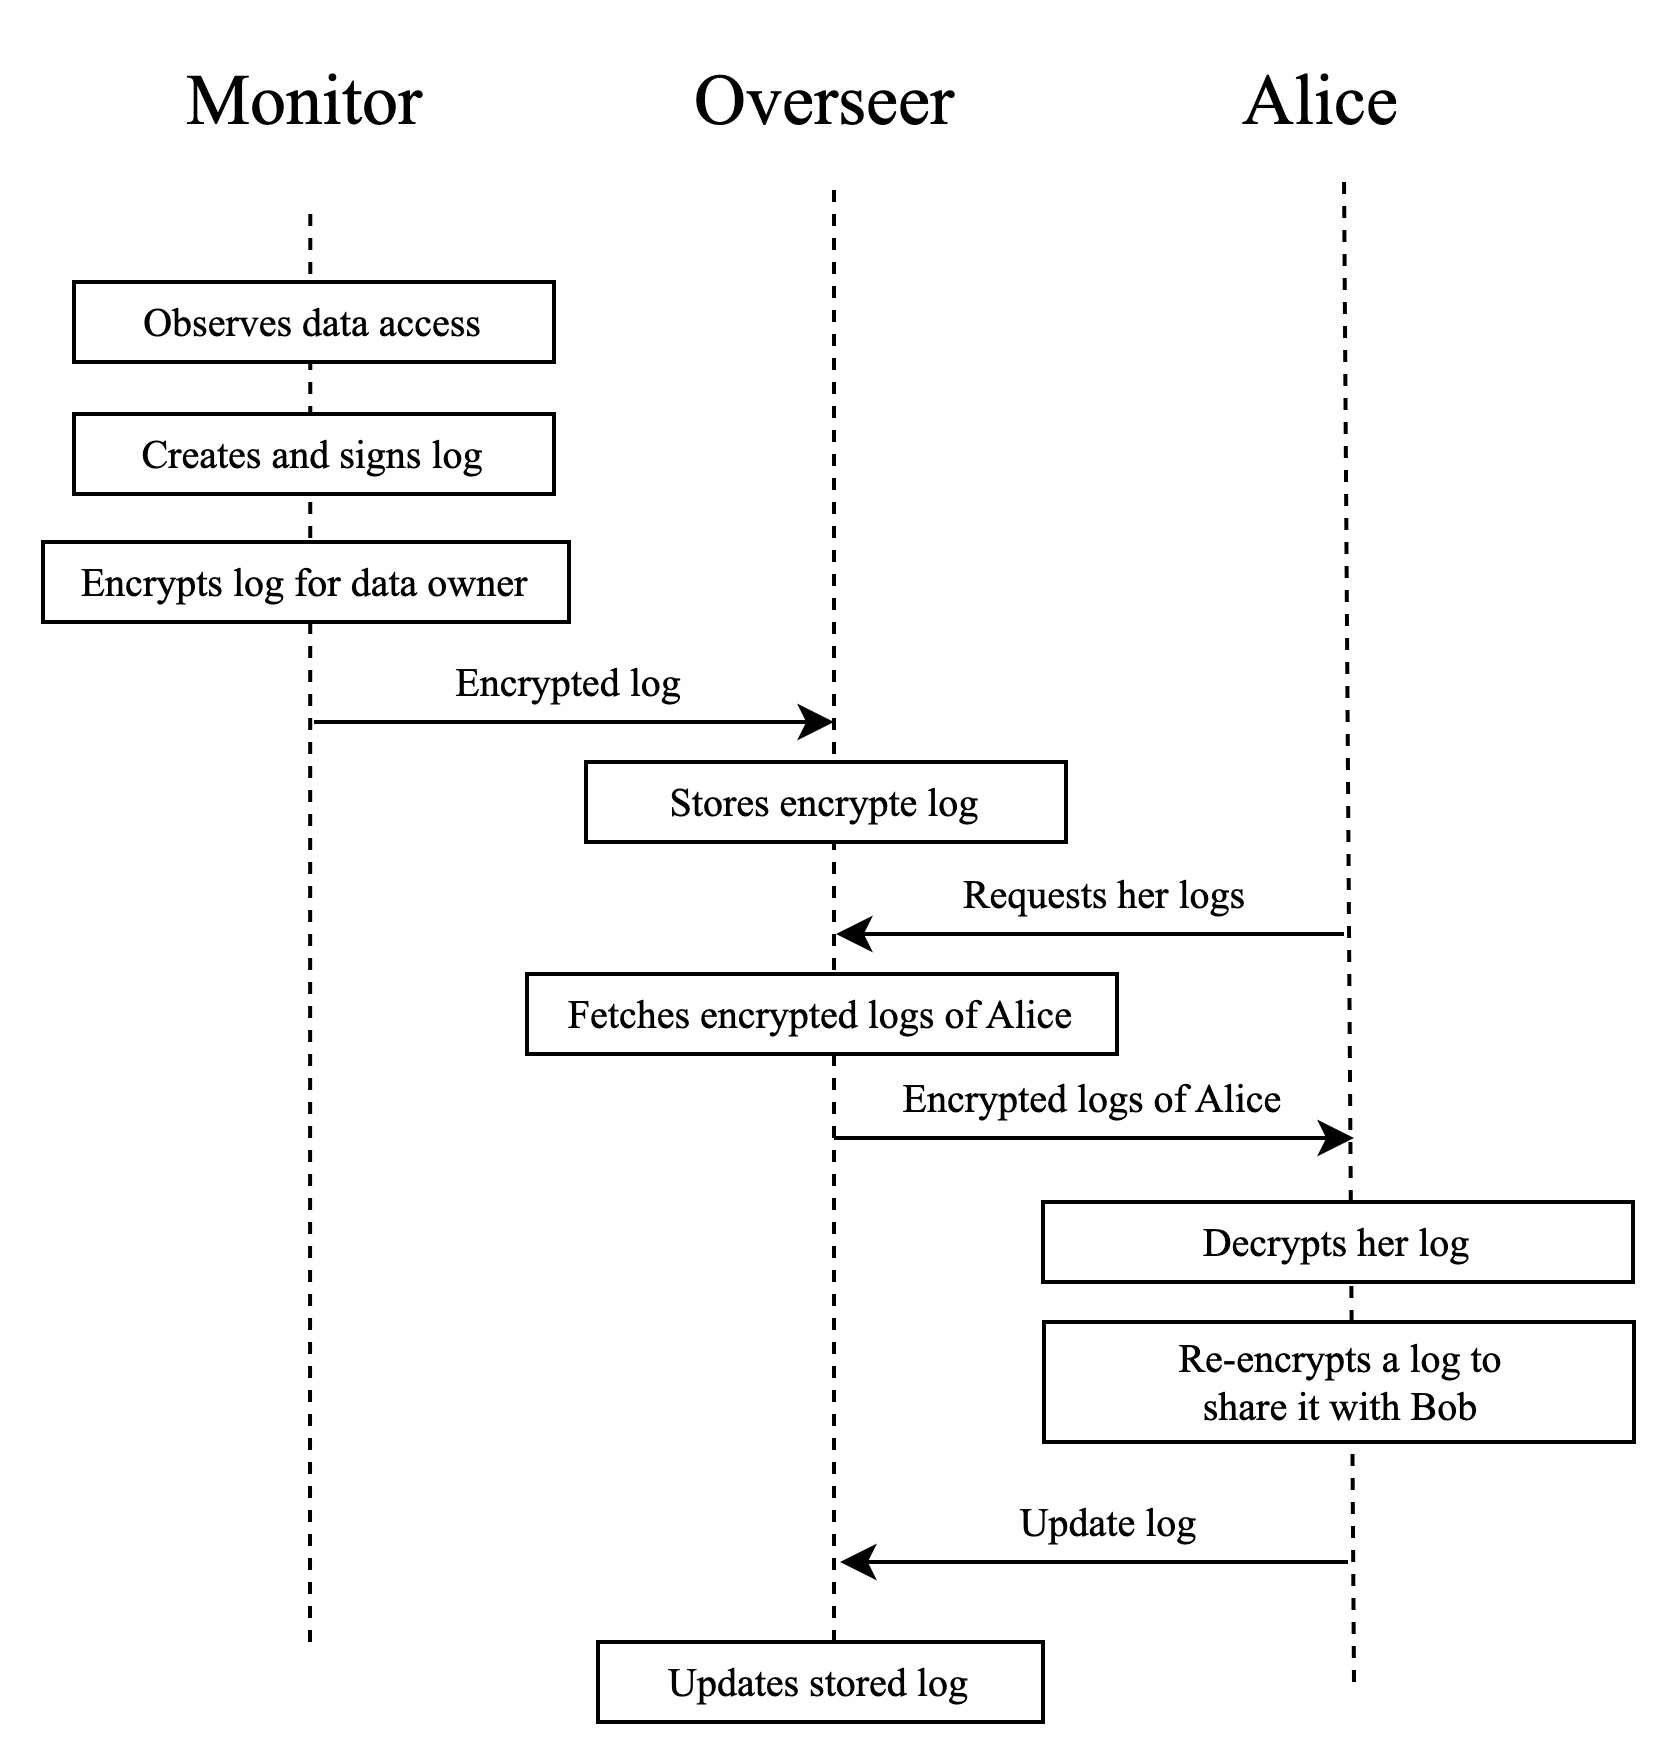
\includegraphics[width=10cm]{../img/05/overview.jpg}
    \centering
    \caption{
        A example that visualizes the performed tasks and data flows when encrypting and sharing logs in the toolchain.
        The monitor creates a log and encrypts it for Alice.
        Alice decides to share the log with Bob.
        Therefore, Alice re-encrypts the log and updates it in the Overseer.
    }
    \label{fig:protocol-overview}
\end{figure}

\section{General considerations}
\label{sec:protocol-considerations}
In this section, general design considerations for the protocol are discussed.
Section~\ref{sec:sign-and-encrypt} evaluates the secure combination of encryption and authentication mechanisms.
To design a practical and efficient protocol, intermediate servers are dependent on metadata.
This is elaborated in section~\ref{sec:metadata}.
Finally, section~\ref{sec:jose-protocol} illustrates how the \textit{JOSE} standard can be used to practically implement the protocol.

\subsection{Secure application of encryption and authentication}
\label{sec:sign-and-encrypt}
In general, the protocol sends encrypted data (containing a log) to a set of recipients.
The recipients must verify the authenticity of the encrypted data because only the owner or the monitor of a log can encrypt.
Thus, the creator of an encrypted log is required to cryptographically sign the sent data.
This arises the question, if encrypted data should be signed (\textit{encrypt-then-sign}) or if signed data should be encrypted (\textit{sign-then-encrypt}).
In general, the \textit{encrypt-then-sign} approach is considered less secure because a malicious entity could simply stripe the signature and sign the ciphertext using its own secret key~\cite{Davis2001}.
This might lead to unintended flaws in the resulting protocol~\cite[section~11.2]{Jones2015a}.

The naive \textit{sign-then-encrypt} approach, however, suffers from surreptitious forwarding (details in section~\ref{sec:surreptitious-forwarding}). 
It can be mitigated by explicitly signing the intended recipients.
This allows a recipient to ensure that the data was intentionally encrypted for him or her by the claimed creator.~\cite{Davis2001}

For the protocol designed in the context of this thesis, those considerations have the following implications:
\begin{enumerate}
    \item 
    The creator signs the log along with the set of recipients.
    Please note that the log itself is also a signed data structure.
    The log must always be signed by the monitor specified within the log to avoid the forgery of logs.
    The signature of the creator ensures that unauthorized sharing operations can be detected.
    \item The signed data is then encrypted for the specified recipients.
\end{enumerate}


\subsection{Metadata}
\label{sec:metadata}
The logs which are exchanged between users are always encrypted.
From the perspective of intermediate servers, this has problematic consequences affecting the performance of the toolchain.
Consider the scenario where servers do not learn anything from the ciphertext because no metadata is attached.
Specifically, they do not know which users have access to a log because the intended recipients are only accessible after decryption (the server can not decrypt due to E2EE).
This introduces the following practical problems:
\begin{enumerate}
    \item 
    Consider that Alice requests the logs concerning her.
    The server can not associate logs with users.
    Thus, the server must reply with all logs stored in the system.
    As a consequence, Alice receives many logs that she can not decrypt.
    Since the raw cipher does not tell her which logs are intended for her, Alice must try to decrypt all logs to find the logs encrypted under her public key.
    This is very inefficient and requires a lot of computational power.
    To avoid this, the set of recipients must be attached as metadata to the encrypted log.
    \item 
    Consider Alice to be a data owner.
    Alice wants to share her log with Bob.
    Before the sharing process starts, the encrypted log is stored in the server.
    Alice re-encrypts the log under the public key of Bob.
    She authenticates against the server and tries to update the stored log in the server.
    The server, however, does not know if Alice is the legitimate owner of the stored log.
    Thus, the server does not allow Alice to update the stored log.
    To avoid this, the server must know the identity of the data owner of a log.
    This can be realized by attaching the identity of the owner as metadata to the encrypted log.
\end{enumerate}
To avoid these problems, the set of receivers and the identity of the data owner need to be accessible without decryption.
This data can be interpreted as routing information and must be attached as metadata to the encrypted logs.
Please note that this implies that the data sent over the insecure network contains the set of recipients twice (once in the metadata and once within the encrypted data).

\subsection{Realization via JOSE}
\label{sec:jose-protocol}

The designed protocol internally uses the \textit{JSON Object Signing and Encryption} standard (\textit{JOSE})~\cite{Barnes2014}.
Details about it can be found in section~\ref{sec:jose}.
The \textit{JOSE} standard defines algorithms to compute \textit{JWS} tokens that contain cryptographically signed data.
It also defines algorithms to produce encrypted \textit{JWE} tokens via hybrid encryption.
Since \textit{JWS} and \textit{JWE} tokens can be nested into each other they can be used to realize the desired protocol:
\begin{enumerate}
    \item 
    A log is a \textit{JWS} token signed by the monitor.
    \item 
    To encrypt a log, the creator computes a \textit{JWS} token which contains the log as a nested token.
    The token additionally contains the set of intended recipients.
    This outer \textit{JWS} token is called a shared log in the context of this protocol.
    See figure~\ref{fig:nested-jws} for a visualization of the nested tokens.
    \item
    The shared log is finally encrypted to obtain a \textit{JWE} token.
    This token also contains the unencrypted metadata within its protected header.
\end{enumerate}


\begin{figure}[h!]
    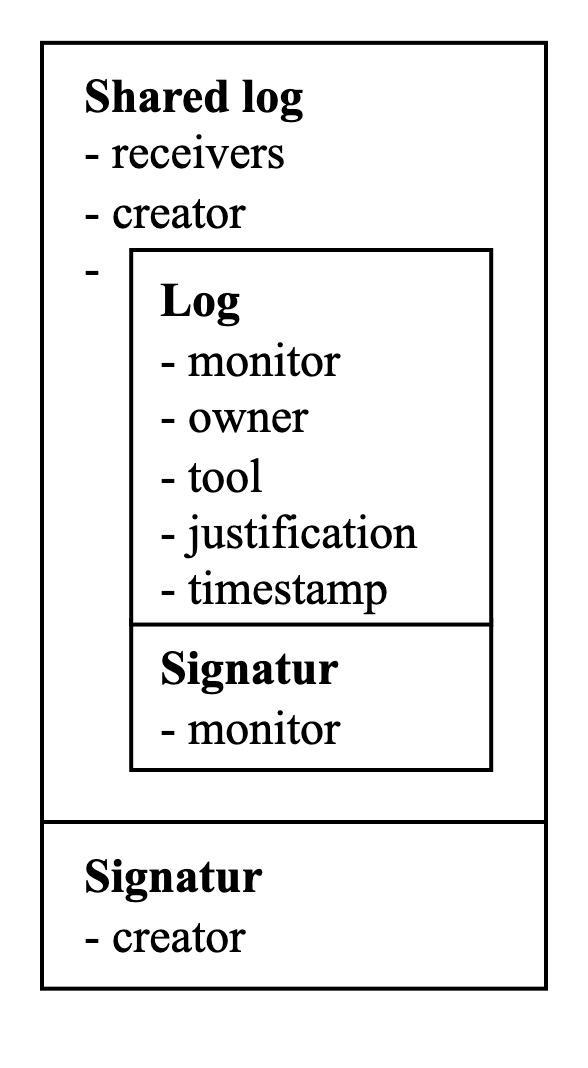
\includegraphics[width=4cm]{../img/05/nested_jws.jpg}
    \centering
    \caption{A log is a \textit{JWS} token signed by the monitor. A shared log is a \textit{JWS} token that contains a nested log. It is signed by the entity creating the shared log (this is either the monitor or the owner of the log).}
    \label{fig:nested-jws}
\end{figure}




\section{Creating logs}
\label{sec:signing}
A log is represented by a \textit{JWS} token.
It contains the identity of the owner, the identity of the monitor and further information which are relevant to identify the data access (see figure~\ref{fig:nested-jws}).
To avoid malicious data owners manipulating or creating new logs, each log needs to be signed by the monitor specified within the log.
To create a \textit{JWS} token, the monitor requires access to its private signing key.
The log is later used as input for the encryption algorithm.
This construction allows users decrypting a log to verify if the provided log was indeed created by the claimed monitor.

\section{Encrypting logs}\label{sec:encrypting}

The encryption algorithm requires two input parameters: A log and the set of users who are allowed to access the log.
It can be performed either by a monitor or the data owner.
A monitor initially encrypts the log for the data owner.
The data owner might decide to share or revoke access to a log for users.
This requires the re-encryption of the log.
The encryption algorithm outputs a JWE token which can be decrypted by the specified users.

Internally, the encryption algorithm creates another \textit{JWS} token.
It is called a shared log because it contains a nested log with additional sharing information (see figure~\ref{fig:nested-jws}).
Besides the set of recipients, it contains the identity of the creator.
The latter allows a decrypting user to download the public key of the creator which is used to verify the shared log.
The set of recipients is included to mitigate surreptitious forwarding (details in section~\ref{sec:sign-and-encrypt}).

Once the  shared log is created, it is used to compute the final \textit{JWE} token.
This is achieved by passing the encoded shared log as plaintext into the JWE encryption algorithm.
The set of recipients and the identity of the owner are passed as metadata into the protected header of the JWE.
The choice of used algorithms to encrypt the data implies hybrid encryption:
The plaintext is encrypted with the authenticated encryption algorithm \verb|A256GCM| (symmetric encryption via 256-bit AES in Galois/Counter Mode).
The applied key-wrapping algorithm is \verb|ECDH-ES+A256KW|.
It is responsible for encrypting the symmetric key for authorized users (asymmetric encryption).
This algorithm establishes a Diffie-Hellman secret between the sender and receiver which is used to symmetrically encrypt the symmetric key using AES.
Details about this approach can be found in \cite[100]{Barker2017}.
Both algorithms are specified by the JSON Web Algorithm (JWA) specification~\cite{Jones2015}.
The whole encryption process is depicted in detail in the appendix~\ref{app:encryption}.

\section{Decrypting logs}\label{sec:decrypting}

The decryption algorithm takes a JWE token and a private decryption key as input.
To verify the \textit{JWS} tokens encoded within the JWE token, this algorithm needs to be able to dynamically resolve the identities of users to their public keys.

First of all, the JWE token is parsed into its ciphertext, header and encrypted keys.
The JWE-decryption algorithm is then applied to the JWE token.
This decrypts the ciphertext using the passed private decryption key.
To be more precise, it tries to decrypt any of the encrypted keys.
If this succeeds, the symmetric encryption key is accessible.
This allows the decryption of the symmetric ciphertext which restores the shared log.
No decryption is necessary to access the metadata because is stored in the protected header of the JWE.
If the decryption is successful, the decrypting user has access to the shared log and the metadata.
Multiple validations are necessary to ensure that the protocol is used correctly.
If any of them fails the decryption must be aborted.
\begin{enumerate}
    \item 
    The signature of the obtained shared log (\textit{JWS} token) must be validated.
    To do so, the decrypting user needs to download the public key of the creator specified in the shared log.
    If the verification of the signatures succeeds, the decrypting user can be sure that the claimed creator indeed signed the shared log.
    \item
    The signature of the nested log (\textit{JWS} token) must be validated.
    Again, the public key of the specified monitor needs to be downloaded.
    If the verification of the signatures succeeds, the decrypting user can be sure that the claimed monitor indeed signed the log.
    \item
    The metadata includes the set of recipients.
    The shared log also includes this information.
    Only if both sets are equal the token was not modified during transit.
    \item
    The user applying the decryption must be part of the set of recipients.
    If this is true, the user can ensure that the creator intended to share the log with him or her.
    \item
    The owner specified in the metadata must be equal to the owner specified in the log.
    Only if both are equal the token was not modified during transit.
    \item
    The log specifies the owner and the monitor of the log.
    The shared log specifies the creator of the encrypted message.
    The creator must be either the owner or the monitor of the log.
    If the creator is equal to the monitor of the log, the monitor encrypted the message for the data owner.
    In this case, the data owner must be the user decrypting the data.
    The set of recipients must only contain the identity of the data owner because the monitor is not allowed to encrypt the log for other users.

    If the creator is equal to the owner of the log, the owner shared the log with other users.
    In this case, the set of recipients can be arbitrary.
\end{enumerate}
If all those validations succeed the log can be trusted.
A visualization of the decryption process can be found in the appendix~\ref{app:encryption}


\end{document}
